\documentclass[a4paper, 12pt]{article}

\usepackage[portuges]{babel}
\usepackage[utf8]{inputenc}
\usepackage{amsmath}
\usepackage{indentfirst}
\usepackage{graphicx}
\usepackage{multicol,lipsum}
% Code
\usepackage{listings}
\usepackage{xcolor}

\definecolor{codegreen}{rgb}{0,0.6,0}
\definecolor{codegray}{rgb}{0.5,0.5,0.5}
\definecolor{codepurple}{rgb}{0.8,0,0.2}
\definecolor{backcolour}{rgb}{.95,.95,1}

\lstdefinestyle{mystyle}{
    backgroundcolor=\color{backcolour},   
    commentstyle=\color{codegreen},
    keywordstyle=\color{blue},
    numberstyle=\tiny\color{codegray},
    stringstyle=\color{codepurple},
    basicstyle=\ttfamily\footnotesize,
    breakatwhitespace=false,         
    breaklines=true,                 
    captionpos=b,                    
    keepspaces=true,                 
    numbers=left,                    
    numbersep=5pt,                  
    showspaces=false,                
    showstringspaces=false,
    showtabs=false,                  
    tabsize=2
}

\lstset{style=mystyle}

\usepackage{qrcode,hyperref}

\begin{document}
%\maketitle

\begin{titlepage}
	\begin{center}
	
	%\begin{figure}[!ht]
	%\centering
	%\includegraphics[width=2cm]{c:/ufba.jpg}
	%\end{figure}

		\Huge{Centro Universitário Instituto de Educação Superior de Brasília}\\
		\large{Departamento de Pós graduação}\\ 
		\large{Especialização em Big Data, BI e Analytics Aplicados aos Negócios}\\ 
		\vspace{12pt}
        \vspace{70pt}
        \textbf{\LARGE{Atividade Ativa}}\\
		%\title{{\large{Título}}}
		\vspace{3,5cm}
	\end{center}
	
	\begin{flushleft}
		\begin{tabbing}
			Aluna: Mariana Borges de Sampaio \\
			Professor: Marco Araujo\\
			Disciplina: Aplicação de dados direta \\
	\end{tabbing}
 \end{flushleft}
	\vspace{1cm}
	
	\begin{center}
		\vspace{\fill}
			 Junho\\
		 2024
			\end{center}
\end{titlepage}
%%%%%%%%%%%%%%%%%%%%%%%%%%%%%%%%%%%%%%%%%%%%%%%%%%%%%%%%%%%

% % % % % % % % %FOLHA DE ROSTO % % % % % % % % % %

\begin{titlepage}
	\begin{center}
	
	%\begin{figure}[!ht]
	%\centering
	%\includegraphics[width=2cm]{c:/ufba.jpg}
	%\end{figure}

		\Huge{Centro Universitário Instituto de Educação Superior de Brasília}\\
		\large{Departamento de Pós graduação}\\ 
		\large{Especialização em Big Data, BI e Analytics Aplicados aos Negócios}\\ 
\vspace{12pt}
        
        \vspace{70pt}
        
		\textbf{\LARGE{Atividade Ativa}}
		\title{\large{Título}}
	%	\large{Modelo\\
     %   		Validação do modelo clássico}
			
	\end{center}
\vspace{1,5cm}
	
	\begin{flushright}

   \begin{list}{}{
      \setlength{\leftmargin}{4.5cm}
      \setlength{\rightmargin}{0cm}
      \setlength{\labelwidth}{0pt}
      \setlength{\labelsep}{\leftmargin}}

      \item Relatório do Atividade Ativa da disciplina de Aplicação de dados direta.
      \begin{list}{}{
      \setlength{\leftmargin}{0cm}
      \setlength{\rightmargin}{0cm}
      \setlength{\labelwidth}{0pt}
      \setlength{\labelsep}{\leftmargin}}

			\item Aluna: Mariana Borges de Sampaio \
            \item Professor: Marco Araujo \

      \end{list}
   \end{list}
\end{flushright}
\vspace{1cm}
\begin{center}
		\vspace{\fill}
		 Junho\\
		 2024
			\end{center}
\end{titlepage}
\newpage
% % % % % % % % % % % % % % % % % % % % % % % % % %
\newpage
\tableofcontents
\thispagestyle{empty}

\newpage
\pagenumbering{arabic}
% % % % % % % % % % % % % % % % % % % % % % % % % % %
\section{Introdução}
Este trabalho tem como intuito apresentar a reprodução de um histograma que foi gerado utilizando a biblioteca pandas do python. De forma que para isso será utilizada a IDE visual studio code, com a instalação da extensão jupyter notebook, que consiste em uma IDE do python. 

Para este trabalho foi utilizado o conjunto de dados sobre acidentes registrados na concessionária RioSP, disponível no dados abertos da ANTT (Agência Nacional de Transportes Terrestres). 
Este conjunto como demais outros conjuntos podem ser encontrados no site: https://dados.antt.gov.br.

Neste trabalho alguns tópicos relacionados a programação e análise de dados devem ser obtidos através do desenvolvimento. Com isso serão apresentados os seguintes itens a fim de comprovar o uso correto desses tópicos:
\begin{itemize}
    \item Utilizar o ambiente de desenvolvimento adequadamente;
    \item Importar as bibliotecas necessárias;
    \item Realizar a análise de dados em python;
    \item Plotar gráficos, no caso, o histograma;
    \item Desenvolvimento de código em python.
\end{itemize}

\newpage
\section{Desenvolvimento}

Inicialmente é necessário fazer a importação da biblioteca necessária para o ambiente de desenvolvimento. A partir disso é possível começar a desenvolver o código para que sejam produzidas as análises necessárias e por fim realizar a plotagem do histograma.
\begin{tabular}{ccc}
\end{tabular}

\begin{lstlisting} 
import pandas as pd 
import numpy as np
import matplotlib.pyplot as plt 
\end{lstlisting}

Tendo o conjunto de dados armazenado na máquina é necessário acessá-lo no código e iniciar a análise de dados.

\subsection{Código}

\begin{tabular}{ccc}
\end{tabular}

\begin{lstlisting} 
import pandas as pd 
import numpy as np
import matplotlib.pyplot as plt 

file = pd.read_csv('demostrativo_acidentes_riosp.csv',encoding='latin1', on_bad_lines='skip',sep =';')
display(file)

file.info()

file['automovel'].hist(bins=5,color='skyblue',edgecolor='grey')
plt.xlabel('automovel')
plt.ylabel('frequencia')
plt.title('Histograma de automoveis envolvidos em acidentes na RioSP')
plt.show()
\end{lstlisting}

Como saída deste código, tem-se o seguinte histograma plotado.

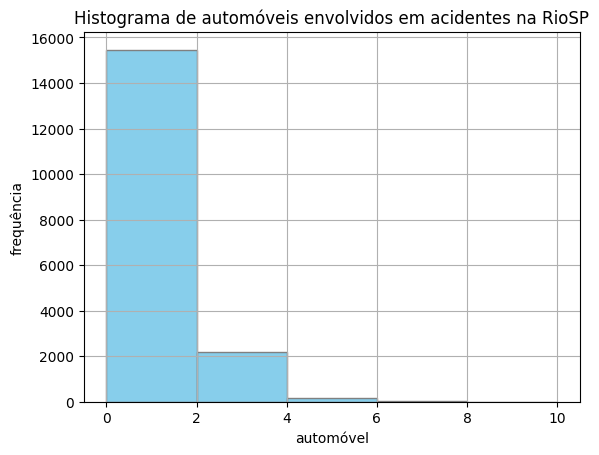
\includegraphics[scale=0.7]{output.png}

De forma que é possível analisar que a frequência da quantidade de automóveis que são envolvidos nos acidentes é de 0 a 2. Seguido de uma segunda maior frequência de 2 a 4 carros envolvidos e como menor frequência, tem-se de 4 a 6 carros envolvidos no acidente. 

Esse mesmo histograma pode ser plotado utilizando a biblioteca seaborn. Para isso é necessárias algumas modificações na leitura do arquivo.


\begin{tabular}{ccc}
\end{tabular}

\begin{lstlisting} 
# Histograma utilizando o seaborn
import seaborn as sns
import pandas as pd

%matplotlib inline
file = pd.read_csv('demostrativo_acidentes_riosp.csv',encoding='latin1', on_bad_lines='skip',sep =';')
sns.displot(file['automovel'])
sns.displot(file['automovel'], kde=False)

\end{lstlisting}

Como saída deste código, tem-se o seguinte histograma plotado.

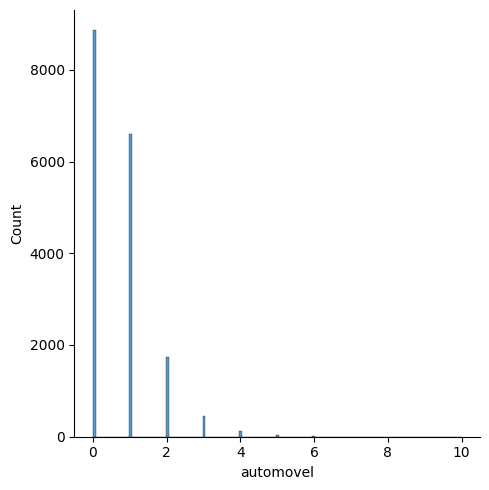
\includegraphics[scale=0.7]{output02.png}

Uma outra informação que pode ser obtida através do histograma são os trechos que tiveram maior quantidade de acidentes registrados na base de dados que está sendo analisada. O código utilizado se encontra abaixo:


\begin{tabular}{ccc}
\end{tabular}

\begin{lstlisting} 
# Histograma dos trechos com acidentes na RioSP
import pandas as pd 
import numpy as np
import matplotlib.pyplot as plt

file = pd.read_csv('demostrativo_acidentes_riosp.csv',encoding='latin1', on_bad_lines='skip',sep =';')
display(file)

file['trecho'].hist(bins=5,color='purple',edgecolor='black')
plt.xlabel('trecho')
plt.ylabel('frequencia')
plt.title('Histograma dos trechos com mais cidentes na RioSP')
plt.show()
\end{lstlisting}
Como saída deste código, tem-se o seguinte histograma plotado.

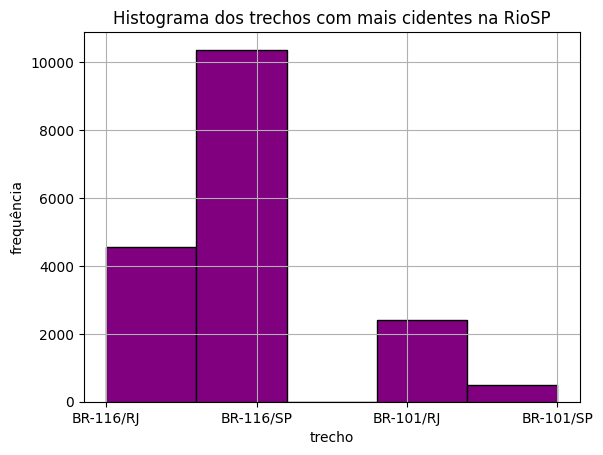
\includegraphics[scale=0.7]{output03.png}

A partir desse gráfico pode ser observado que os trechos com maior frequência de acidentes registrados na base de dados analisada foram no trecho BR-116/SP, seguido da BR-116/RJ, BR-101/RJ e a BR-101/SP.

Fazendo esse mesmo gráfico utilizando a biblioteca seaborn, tem-se o seguinte código:

\begin{tabular}{ccc}
\end{tabular}

\begin{lstlisting} 
# Histograma utilizando o seaborn
import seaborn as sns
import pandas as pd

%matplotlib inline
file = pd.read_csv('demostrativo_acidentes_riosp.csv',encoding='latin1', on_bad_lines='skip',sep =';')
sns.displot(file['trecho'], color='skyblue')
sns.displot(file['trecho'], kde=True,color='skyblue')

\end{lstlisting}

Como saída deste código, tem-se o seguinte histograma plotado.

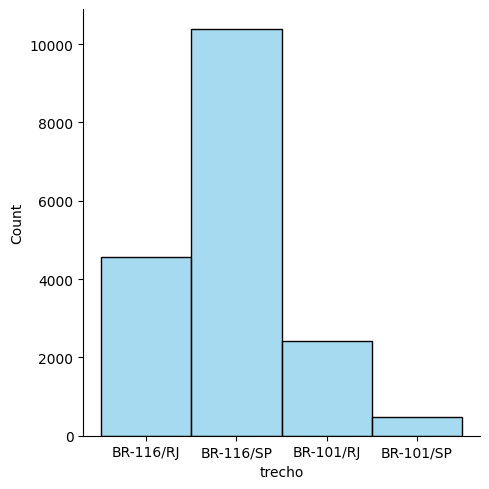
\includegraphics[scale=0.7]{output04.png}

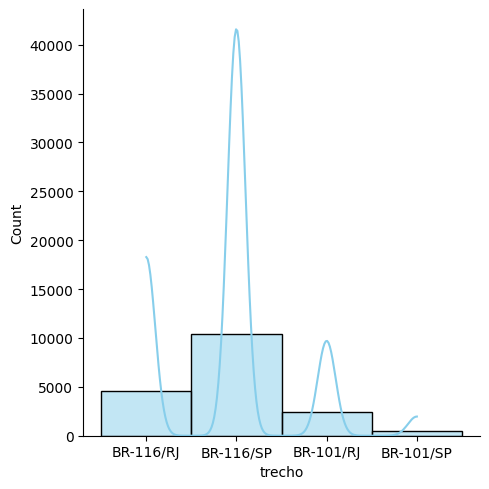
\includegraphics[scale=0.7]{output05.png}


Uma diferença desse código está na linha 8. Esta linha evidencia um parâmetro que não havia sido utilizado anteriormente que é o 'kde = True'. Com esse parâmetro é traçada uma linha que é a estimativa da linha gaussiana. De forma que a escala de frequência também é alterada quando se tem esse escala adicionada. 

A linha gaussiana corresponde a distribuição normal, curva de Gauss. Ela é uma distribuição padronizada com uma média e o desvio padrão e tem sido muito utilizada na análise exploratória de dados. Logo, ao ver a linha gaussiana no histograma isso indica a representação esperada dos dados caso eles seguissem uma distribuição normal. De forma que com a aplicação da linha gaussiana é possível entender onde estão concentrados a maioria dos valores que estão sendo analisados da base de dados em questão.

\newpage
\section{Considerações finais}


Por fim, é possível observar que analisar os dados utilizando python pode ser extremamente relevante para quem trabalha com a área de dados. Pois existem recursos que podem ser mais explorados através da programação que por vezes apenas com a análise do excel ou csv são mais superficiais. 

Sendo assim o conhecimento de linguagens de programação podem ser bem usufruídos quando relacionados a área em que se está trabalhando. Além disso, vale ressaltar que a linguagem de programação vem crescendo cada vez mais nas mais diversas áreas, como na análise de dados, ciência de dados, estudos de redes neurais , inteligência artificial dentre outras áreas.

Os arquivos e códigos feitos foram adicionados ao github no seguinte link: https://github.com/sampaiomariana/histogram. O relatório foi feito utilizando Latex e como editor online foi utilizado o Overleaf.

\newpage
\addcontentsline{toc}{section}{Bibliografia}
\section*{Bibliografia}
\footnotesize{

\noindent ELMASRI, Ramez e NAVATHE, Shamkant B. Sistemas de Banco de Dados. Pearson Addison Wesley. 6a Edição, 2011.\\

\noindent TEAM, The Matplotlib Development. Matplotlib 3.9.0 documentation. 2024. Disponível em: https://matplotlib.org/stable/index.html. Acesso em: 12 jun. 2024.\\

\noindent  INC, Numfocus. Pandas documentation. 2024. Disponível em: https://pandas.pydata.org/docs/. Acesso em: 12 jun. 2024. \\

\noindent  MARQUES, Leonardo Torres. Preparação e análise exploratória de dados: histogramas com seaborn. Histogramas com seaborn. 2024. \\

\noindent  UFSC. Distribuição Normal (Gaussiana). Disponível em: https://www.inf.ufsc.br/~andre.zibetti/probabilidade/normal.html. Acesso em: 15 jun. 2024.
\\
}
\end{document}



